% Options for packages loaded elsewhere
\PassOptionsToPackage{unicode}{hyperref}
\PassOptionsToPackage{hyphens}{url}
%
\documentclass[
]{article}
\usepackage{lmodern}
\usepackage{amssymb,amsmath}
\usepackage{ifxetex,ifluatex}
\ifnum 0\ifxetex 1\fi\ifluatex 1\fi=0 % if pdftex
  \usepackage[T1]{fontenc}
  \usepackage[utf8]{inputenc}
  \usepackage{textcomp} % provide euro and other symbols
\else % if luatex or xetex
  \usepackage{unicode-math}
  \defaultfontfeatures{Scale=MatchLowercase}
  \defaultfontfeatures[\rmfamily]{Ligatures=TeX,Scale=1}
  \setsansfont[]{Calibri Light}
\fi
% Use upquote if available, for straight quotes in verbatim environments
\IfFileExists{upquote.sty}{\usepackage{upquote}}{}
\IfFileExists{microtype.sty}{% use microtype if available
  \usepackage[]{microtype}
  \UseMicrotypeSet[protrusion]{basicmath} % disable protrusion for tt fonts
}{}
\makeatletter
\@ifundefined{KOMAClassName}{% if non-KOMA class
  \IfFileExists{parskip.sty}{%
    \usepackage{parskip}
  }{% else
    \setlength{\parindent}{0pt}
    \setlength{\parskip}{6pt plus 2pt minus 1pt}}
}{% if KOMA class
  \KOMAoptions{parskip=half}}
\makeatother
\usepackage{xcolor}
\IfFileExists{xurl.sty}{\usepackage{xurl}}{} % add URL line breaks if available
\IfFileExists{bookmark.sty}{\usepackage{bookmark}}{\usepackage{hyperref}}
\hypersetup{
  pdftitle={Michael Barrowman, MSci},
  hidelinks,
  pdfcreator={LaTeX via pandoc}}
\urlstyle{same} % disable monospaced font for URLs
\usepackage[left=1cm,right=1cm,top=1cm,bottom=2cm]{geometry}
\usepackage{graphicx}
\makeatletter
\def\maxwidth{\ifdim\Gin@nat@width>\linewidth\linewidth\else\Gin@nat@width\fi}
\def\maxheight{\ifdim\Gin@nat@height>\textheight\textheight\else\Gin@nat@height\fi}
\makeatother
% Scale images if necessary, so that they will not overflow the page
% margins by default, and it is still possible to overwrite the defaults
% using explicit options in \includegraphics[width, height, ...]{}
\setkeys{Gin}{width=\maxwidth,height=\maxheight,keepaspectratio}
% Set default figure placement to htbp
\makeatletter
\def\fps@figure{htbp}
\makeatother
\setlength{\emergencystretch}{3em} % prevent overfull lines
\providecommand{\tightlist}{%
  \setlength{\itemsep}{0pt}\setlength{\parskip}{0pt}}
\setcounter{secnumdepth}{-\maxdimen} % remove section numbering
\newenvironment{brow}{}{}
\newenvironment{trow}{}{}
\newenvironment{leftpanel}{}{}
\newenvironment{footer}{}{}

\usepackage{booktabs}
\usepackage{longtable}
\usepackage{array}
\usepackage{multirow}
\usepackage{wrapfig}
\usepackage{float}
\usepackage{colortbl}
\usepackage{pdflscape}
\usepackage{tabu}
\usepackage{threeparttable}
\usepackage{threeparttablex}
\usepackage[normalem]{ulem}
\usepackage{makecell}
\usepackage{xcolor}
\usepackage{multicol}
\usepackage{hyperref}

\title{Michael Barrowman, MSci}
\author{}
\date{\vspace{-2.5em}}

\begin{document}
\maketitle

\newcommand{\bcols}{\begin{multicols}{2}}
\newcommand{\ecols}{\end{multicols} }
\newcommand{\iimg}[1]{\includegraphics[height=2ex]{#1}}
\renewcommand{\arraystretch}{1.7}

\begin{brow}

\begin{trow}

\setlength{\columnsep}{-2.5cm}
\def\addlinespace{}

\begin{multicols}{2}

\begin{leftpanel}

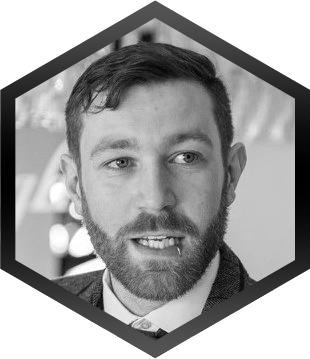
\includegraphics[width=0.3\textwidth]{img/ProfileHex}

\begin{tabular}{l}
\toprule

\includegraphics[height=2ex]{ img/logos/tel-logo.png} \href{ tel:+447467456803}{ (+44) 07467 456 803}\\

\includegraphics[height=2ex]{ img/logos/email-logo.png} \href{ mailto:myko101ab@gmail.com}{ myko101ab@gmail.com}\\

\includegraphics[height=2ex]{ img/logos/twitter-logo.png} \href{ https://twitter.com/MyKo101ab}{ @MyKo101ab}\\

\includegraphics[height=2ex]{ img/logos/github-logo.png} \href{ https://github.com/MyKo101}{ MyKo101}\\

\includegraphics[height=2ex]{ img/logos/orcid-logo.png} \href{ https://orcid.org/0000-0003-0718-4482}{ 0000-0003-0718-4482}\\


\includegraphics[height=2ex]{ img/logos/linkedin-logo.png} \href{ https://www.linkedin.com/in/michael-barrowman-0403a960/}{ michael-barrowman}\\

\includegraphics[height=2ex]{ img/logos/location-logo.png} \href{ https://www.google.com/maps/place/Newton-le-Willows/@53.4584287,-2.6730042}{ Newton-Le-Willows}\\

\includegraphics[height=2ex]{ img/logos/internet-logo.png} \href{ https://MichaelBarrowman.co.uk/CV/index.html}{ MichaelBarrowman.co.uk/CV}\\
\bottomrule
\end{tabular}

\end{leftpanel}

\hypertarget{section}{%
\section{}\label{section}}

\hypertarget{bio}{%
\subsection{Bio}\label{bio}}

\hypertarget{about-me}{%
\subsubsection{About Me}\label{about-me}}

Expert data scientist with a Masters Degree in Mathematics, approaching
completion of a PhD in Medicine with a focus on Statistics. Achievements
include 10\% improvement in effective productivity in examination
marking, the creation of SAPs and SOPs for a pioneering pragmatic
clinical trial and the development and validation of a multi-state
clinical predication model, as well as the methodological advancements
to produce such a model. I have a multitude of published works including
packages in R, where my most recent experience lies, articles in high
impact journals covering methodology and clinical advances. Highly
skilled in data processing, visualisation and model building. Extremely
versatile in language use and flexible in it's application.

\hypertarget{skills}{%
\subsubsection{Skills}\label{skills}}

\mbox{\includegraphics[height=2ex]{ img/logos/r-logo.png} R}\quad\mbox{\includegraphics[height=2ex]{ img/logos/rmarkdown-logo.png} RMarkdown}\quad\mbox{\includegraphics[height=2ex]{ img/logos/latex-logo.png} LaTeX}\quad\mbox{\includegraphics[height=2ex]{ img/logos/spss-logo.png} SPSS}\quad\mbox{\includegraphics[height=2ex]{ img/logos/nvivo-logo.png} NVivo}\quad\mbox{\includegraphics[height=2ex]{ img/logos/git-logo.png} Git}\quad\mbox{
\includegraphics[height=2ex]{ img/logos/github-logo.png} GitHub}\quad\mbox{
\includegraphics[height=2ex]{ img/logos/github-actions-logo.png} GitHub Actions}\quad\mbox{\includegraphics[height=2ex]{ img/logos/html-css-logo.png} HTML/CSS}\quad\mbox{
\includegraphics[height=2ex]{ img/logos/regex-logo.png} Regex}\quad\mbox{
\includegraphics[height=2ex]{ img/logos/python-logo.png} Python}\quad\mbox{
\includegraphics[height=2ex]{ img/logos/sas-logo.png} SAS}\quad\mbox{
\includegraphics[height=2ex]{ img/logos/stata-logo.png} Stata}\quad\mbox{
\includegraphics[height=2ex]{ img/logos/sql-logo.png} SQL}\quad\mbox{
\includegraphics[height=2ex]{ img/logos/microsoft-office-logo.png} Microsoft Office}\quad\mbox{
\includegraphics[height=2ex]{ img/logos/google-suite-logo.png} Google Suite}\quad\mbox{
\includegraphics[height=2ex]{ img/logos/photoshop-logo.png} Photoshop}

\hypertarget{section-1}{%
\subsubsection{}\label{section-1}}

\end{multicols}

\hypertarget{experience}{%
\subsection{Experience}\label{experience}}

\begin{table}[H]
\centering\begin{table}[H]
\centering
\begin{tabular}{>{\raggedright\arraybackslash}p{0.45\textwidth}>{\raggedright\arraybackslash}p{0.45\textwidth}}
\toprule
[0.3em]
\multicolumn{2}{l}{\textit{\textbf{Liverpool John Moores University}}}\\
\hline
\hspace{1em}\textbf{ Maths, Stats \& IT Tutor }, Dec '19 - Present\newline Assisting undergraduate and postgraduate students with Mathematics, Statistics and IT issues relating to their university course, and extending this support to teaching and research staff. Writing and providing tutorial sessions on a variety of subjects and softwares including Microsoft Word, R for Statistics, nVivo for Qualitative Research and SPSS. & \\
[0.3em]
\multicolumn{2}{l}{\textit{\textbf{University of Manchester}}}\\
\hline
\hspace{1em}\textbf{ PhD Student }, Oct '16 - Present\newline The goal of this PhD is to improve the academic knowledge surrounding Multi-State Clinical Prediction Models (MSCPMs). To accomplish this, I am writing articles to solve methodological issues that are yet to be addressed and applying these novel techniques (along with the present literature) to develop and validate an MSCPM to predict outcomes for Chronic Kidney Disease patients. & \textbf{ Lead Statistician }, Jan '17 - Feb '19\newline Working within the University of Manchester, we formed a team of statistical consultants to assist researchers from all levels of the university with their statistical needs, this included help on specific projects and tutorials on various statistical topics. Our efforts helped educate undergraduate students on basic methods to improve their coursework results and provided lecturers and professors with advice and mentoring to focus their research questions and process their results to produce viable academic outputs.\\
\hspace{1em}\textbf{ Research Assistant }, Nov '15 - Sep '16\newline As part of the GetReal consortium, I worked within a multi-national team producing methodological techniques to assist in bridging the gap between efficacy and effectiveness in pragmatic clinical trials. Alongside this methodological work, I was involved in an applied study to assess the generalisability and the risk of a Hawthorn Effect in the Salford Lung Study (SLS), a real-world, pragmatic randomised controlled trial. & \textbf{ Assistant Statistician }, Aug '14 - Apr '15\newline Primarily focused on the deliverables for the SLS. I produced standardised datasets for our pharmaceutical client, ad hoc data analyses and standard operating procedures for the clinical research group. I developed an algorithm utilising a probabilistic model for the merging of pharmacy data with electronic health records sourced from local primary and secondary care data and electronic case report forms provided by the onsite research nurses.\\
[0.3em]
\multicolumn{2}{l}{\textit{\textbf{Brammer UK}}}\\
\hline
\hspace{1em}\textbf{ Data Project Analyst }, Sep '15 - Nov '15\newline Within our team of Data Project Analysts, we were tasked with mass data migration and re-unification. I created a system to automate many processes and accelerate the progress of the migration. & \\
[0.3em]
\multicolumn{2}{l}{\textit{\textbf{AQA}}}\\
\hline
\hspace{1em}\textbf{ Data Analyst }, May '15 - Sep '15\newline Producing business insights and progress reports for examinations results. Coordinated with principal and senior examiners to set grade boundaries based on subject-level knowledge and data derived results. Reprised previous administrative responsibilities to assist other teams within the logistics and production group. & \textbf{ General Assistant }, Jun '13 - Aug '14\newline A wide range of roles, including liaising with internal teams and external examiners to provide support and coordination in order to hit marking deadlines and targets in supervisory, administrative and clerical roles. Managing a large workload of examination tasks and providing insights into the progress of the current series.\\
\bottomrule
\end{tabular}
\end{table}
\end{table}

\hypertarget{software}{%
\subsection{Software}\label{software}}

\begin{table}[H]
\centering
\begin{tabular}{>{\raggedleft\arraybackslash}p{0.1\textwidth}>{\raggedright\arraybackslash}p{0.8\textwidth}}
\toprule
\raisebox{-0.7\height}{
\includegraphics[width=2cm]{ img/logos/typos-logo.png}} & \makecell[tp{0.7\textwidth}]{\textbf{ typos} (R Package) \\  The goal of typos is to provide a flexible warning when commonly mis-typed functions are called. Functions with typing errors will still be evaluated and a warning will be output. It also provides the user with a convenient function to define their own typos. }\\
\bottomrule
\end{tabular}
\end{table}
\begin{table}[H]
\centering
\begin{tabular}{>{\raggedleft\arraybackslash}p{0.8\textwidth}>{\raggedright\arraybackslash}p{0.1\textwidth}}
\toprule
\makecell[tp{0.7\textwidth}]{\textbf{ mutils} (R Package) \\  The goal of mutils is to provide useful functions to make data processing smoother. Most functions contained here are "nifty", rather than "innovative". } & \raisebox{-0.7\height}{
\includegraphics[width=2cm]{ img/logos/mutils-logo.png}}\\
\bottomrule
\end{tabular}
\end{table}
\begin{table}[H]
\centering
\begin{tabular}{>{\raggedleft\arraybackslash}p{0.1\textwidth}>{\raggedright\arraybackslash}p{0.8\textwidth}}
\toprule
\raisebox{-0.7\height}{
\includegraphics[width=2cm]{ img/logos/mpipe-logo.png}} & \makecell[tp{0.7\textwidth}]{\textbf{ mpipe} (R Package) \\  The mpipe package is designed to add extra functionality to the pipeline process in tidyverse style R usage }\\
\bottomrule
\end{tabular}
\end{table}

\hypertarget{publications}{%
\subsection{Publications}\label{publications}}

\begin{table}[H]
\centering
\begin{tabular}{>{\raggedright\arraybackslash}p{0.9\textwidth}}
\toprule
\textbf{MA Barrowman}, N Peek, M Lambie et al, \emph{ How unmeasured confounding in a competing risks setting can affect treatment effect estimates in observational studies }, BMC Medical Research Methodology (2019) doi:10.1186/s12874-019-0808-7\\
\textbf{MA Barrowman}, GP Martin, N Peek et al, \emph{ The Application of Multi-State Methods to Develop Clinical Prediction Models Designed for Clinical Use - A Scoping Review }, OSF (2019) doi:10.17605/OSF.IO/HR6QD\\
A Pate, \textbf{MA Barrowman}, D Webb et al, \emph{ Study investigating the generalisability of a COPD trial based in primary care (Salford Lung Study) and the presence of a Hawthorne effect }, BMJ Open Respiratory Research (2018) doi:10.1136/bmjresp-2018-000339\\
\bottomrule
\end{tabular}
\end{table}

\end{trow}

\begin{footer}

\end{footer}

\end{brow}

\end{document}
